\chapter{Body of my thesis}
\label{chapter:body}
\thispagestyle{myheadings}

% set this to the location of the figures for this chapter. it may
% also want to be ../Figures/2_Body/ or something. make sure that
% it has a trailing directory separator (i.e., '/')!
\graphicspath{{2_Body/Figures/}}

\section{System R}
\label{sec:systemR}
\section{Deep Reinforcement learning}
\label{sec:drl}

Markov decision process(MDP) is used to formalize various types of stochastic processes. In MDPs, the goal of the agent is to make a sequence of actions to optimize/ maximize an objective function. \\
Formally a MDP is a $5-$tuple 
\begin{center}
$\langle S,A,P(s,a),R(s,a), s_0 \rangle $\\
$S \to $ Set of all possible states the agent can be in.\\
$A \to $ Set of all possible actions the agent can take.\\
$P(s,a) \to $ A probability distribution of going to various states given current state and action. $s^{1} \sim P(s,a)$\\
$R(s,a) \to $ Reward for taking action $a$ on state $s$.\\
$s_0 \to $ Describes the initial state of the system/ agent.
\end{center}
The performance of the agent is measured using the rewards collected along the way through various states. So the objective of an MDP is to find a policy $\pi:S\rightarrow A$, a function that maps states to actions, in order to maximize the expected value:-
\begin{center}
    \[ 
    \argmax_{\pi} \mathbb{E} \left[ \sum^{T-1}_{t=0}R(s_{t},a_{t})  \right]
    \] 
    subject to $s_{t+1} = P(s_{t},a_{t}), a_{t} = \pi{s_{t}}$
\end{center}
This method does not reduce the search space, and unlikely greedy solution, this will lead to an optimal solution. This method does not reduce the search space, and unlikely greedy solution, this will lead to an optimal solution.
\par Reinforcement learning(RL) is a technique which optimizes MDPs iteratively, by running a simulation in each iteration and changing the policy to find an optimal one based on the cumulative reward.
\section{Relations}
\label{sec:relations}
A common method/ data structure used to formalize joins
\par \textbf{Query Graph $\to$} A query graph $G$ is an undirected graph, where each relation R is a vertex and each join predicate $\rho$ defines an edge between $2$ vertices. Let $\kappa_G$ denote the number of connected components in $G$
\par A join of relation $R_1, R_2$, in the graph corresponds to remove the vertices $v_{R_1}, v_{R_2}$, replacing them with a vertex $v_{R_1+R_2}$, the edges of the form $(v_{R_1},v) \& (v_{R_2},v)$ are replaced by $(v_{R_1+R_2}, v)$. Note each reduction reduces number of vertices by one, so this process is repeated until there are $\kappa_G$ number of vertices left.
\par \textbf{Join Optimization Problem $\to$} Let $G$ be a query graph and $J$ be a join cost model. Find sequence, $c_1\circ c_2\circ ... \circ c_n$ resulting in $|V| = \kappa_G$ to minimize
\begin{center}
    \[
        \min_{c_1,c_2,...c_n} \sum^{n}_{i=1}J(c_i)
    \] 
    subject to $G_{i+1} = c(G_i)$
\end{center}
Using these definitions, we define a MDP. 
\begin{center}
$\langle \{G_0,G_1,...G_T\},c,P(G,c),-J, G \rangle $\\
\end{center}
We are still not certain about how the cost function $J$ is structured. We are still not certain about how the cost function $J$ is structured. We are still not certain about how the cost function $J$ is structured.

We are still not certain about how the cost function $J$ is structured.












Here goes all the important stuff, likely with a lot of graphics like this:

\begin{figure}[htb]
  \begin{minipage}[t]{0.49\linewidth}\centering
    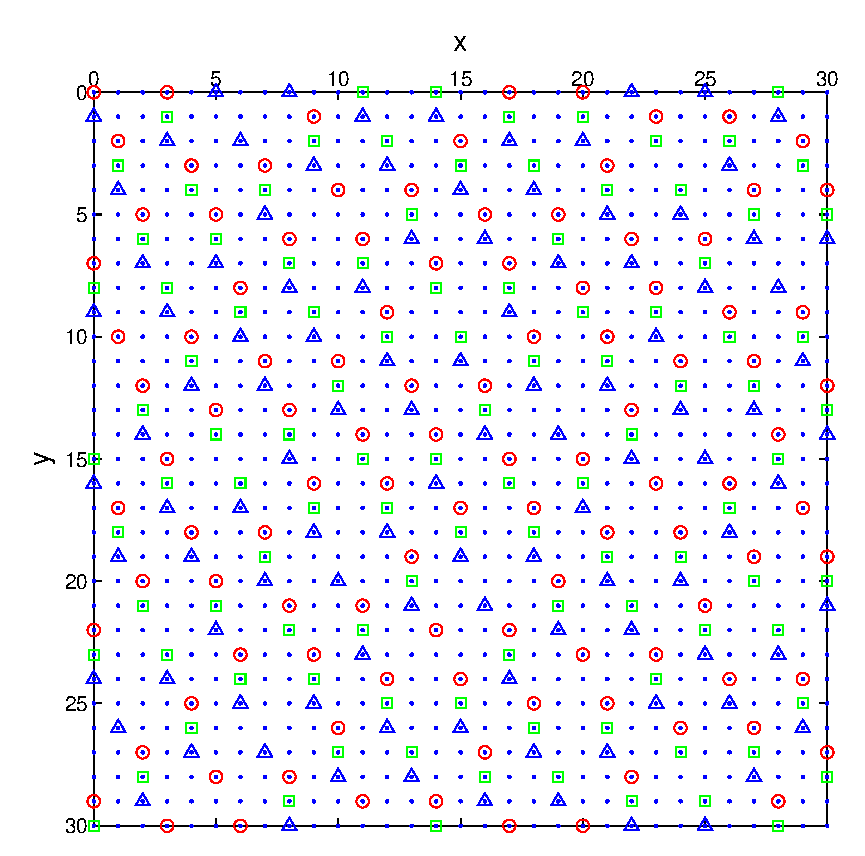
\includegraphics[width=7cm]{figure_sampling_view1.eps}
    \medskip
    \centerline{(a)}
  \end{minipage}\hfill
  \begin{minipage}[t]{0.49\linewidth}\centering
    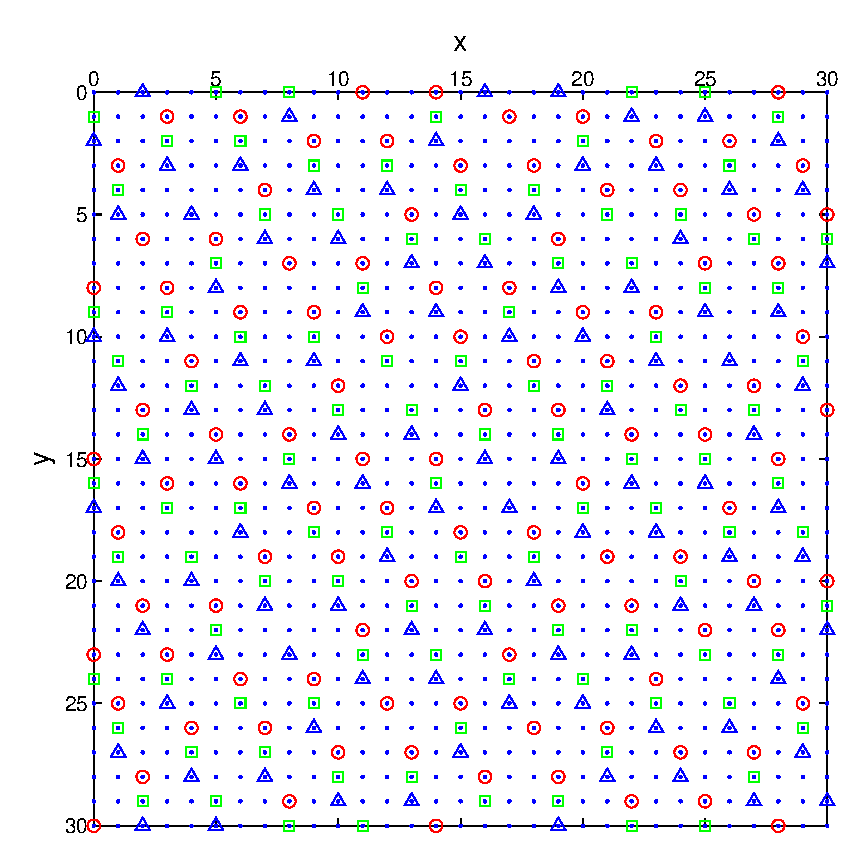
\includegraphics[width=7cm]{figure_sampling_view2.eps}
    \medskip
    \centerline{(b)}
  \end{minipage}
  \caption{Assignment of single-view intensities to RGB components: (a) view
    \#1; and (b) view \#2. }
  \label{fig:Sampling}
\end{figure}

You will also be using a lot of citations. Here is the format required in the dissertation: \cite{lamport1985:latex},\cite{Debr01}.

In all likelihood, you will need to insert tables. See one example on the next page.
\clearpage

\begin{table}[h]
	\caption{Absolute disparity error per pixel for the test data from
		Fig.~\ref{fig:Sampling} and different parameter values. In each experiment one
		parameter is adjusted while other parameters are unchanged.} 
	\centering
	\begin{minipage}[b]{0.30\linewidth}
		\centerline{$\eta=6000$, $\mu=2000$}\smallskip
		\centering
		\begin{tabular}{ccc}
			\hline
			$K$ & $u_1$ & $u_2$\\
			\hline
			3   & 0.52 &0.46\\
			7   & 0.47 &0.43\\
			10  & 0.35 &0.36\\
			12  & 0.37 &0.36\\
			\hline
		\end{tabular}
	\end{minipage}
	%
	\begin{minipage}[b]{0.34\linewidth}
		\centerline{$K=10$, $\mu=2000$}\smallskip
		\centering
		\begin{tabular}{ccc}
			\hline
			$\eta$ & $u_1$ & $u_2$\\
			\hline
			1000&0.54& 0.45\\
			3000&0.43& 0.40\\
			6000&0.35& 0.36\\
			9000&0.37& 0.37\\
			\hline
		\end{tabular}
	\end{minipage}
	%
	\begin{minipage}[b]{0.32\linewidth}
		\centerline{$K=10$, $\eta=6000$}\smallskip
		\centering
		\begin{tabular}{ccc}
			\hline
			$\mu$ & $u_1$ & $u_2$\\
			\hline
			100 &1.00&1.16\\
			1000&0.53&0.47\\
			2000&0.35&0.36\\
			3000&0.44&0.43\\
			\hline
		\end{tabular}
	\end{minipage}
	%
	\label{tab:Parameters}
\end{table}

Of course, there must be a Table of Contents at the beginning of the thesis.